\documentclass[onecolumn,PRD,amsmath,amssymb,aps,nofootinbib,superscriptaddress,11pt]{revtex4-2}

\usepackage{graphicx}
\usepackage{dcolumn}
\usepackage{bm}
\usepackage{hyperref}
\usepackage{color}
\usepackage{setspace}

\begin{document}

\title{The Information-Saturated Bounce: Deriving de Sitter Inflation from the Complete Non-Locality of the MI-Laplacian}

\author{Paul Jarvis}
\email{mrpaulwjarvis@gmail.com}
\affiliation{Independent Researcher, United Kingdom}

\date{\today}

\begin{abstract}
We present a first-principles, coordinate-free mechanism for a cyclic cosmological bounce derived from the spectral dynamics of mutual-information (MI) Laplacians on a relational quantum substrate. By tracking the evolution of the network substrate as it approaches an information-theoretic singularity, we demonstrate that the collapse of spatial locality corresponds to a strict thermodynamic phase transition where the entanglement decay exponent $\alpha \to 0^+$. Numerically evaluating the network's geometric response under volume rescalings, we prove that this maximum saturation limit forces the effective equation of state parameter to converge smoothly and continuously onto the dark energy threshold ($w_{\text{eff}} = -1.0$). Simultaneously, the spectral gap—serving as a proxy for the effective energy density—saturates at a hard algebraic ceiling fixed by the total number of lattice nodes ($\lambda_1 = N$). This invariant cutoff eliminates unphysical density divergences ($\rho \to \infty$), transforming the attractive cosmic crunch into an inherently regularized, gravitationally repulsive de Sitter expansion phase. We demonstrate the structural stability of this fixed-point attractor across disparate non-spatial graph families under extreme multi-channel chaotic noise. Finally, by mapping the Renormalization Group (RG) flow trajectories and numerically extracting their negative $\beta$-functions ($\beta < 0$), we reveal a universal low-dimensional attractor manifold. These results unify microscopic information bounds with cyclic macro-cosmology, demonstrating that Cosmic Inflation is an unavoidable structural consequence of an information-saturated quantum crunch.
\end{abstract}

\maketitle

\setstretch{1.15}

\section{Introduction}
A foundational challenge in modern theoretical cosmology is resolving the unphysical singularity that occurs at the boundary of a collapsing universe. In standard General Relativity, a cosmic crunch compresses matter into a zero-volume point, forcing the macroscopic energy density to diverge toward infinity ($\rho \to \infty$). To circumvent this breakdown of classical spacetime, various frameworks—ranging from Loop Quantum Cosmology to string-inspired braneworlds—postulate ad-hoc fields, high-curvature counter-terms, or external bouncing actions.

In this work, we present a self-contained, coordinate-free alternative. We show that the cosmic bounce is not an added phenomenon but an intrinsic, unavoidable consequence of information-theoretic constraints on a relational quantum substrate. Building on recent models where spacetime geometry emerges from the spectrum of mutual-information (MI) Laplacians, we model a cosmic contraction as an information-theoretic compression phase.

As the available spatial volume shrinks, the microscopic degrees of freedom pack tightly together until they saturate the holographic Bekenstein bound. At this absolute saturation threshold, spatial locality undergoes a fundamental phase transition: the entanglement decay exponent collapses ($\alpha \to 0^+$), transforming the local manifold into a maximally entangled complete graph ($K_N$).

Using exact numerical diagonalization on translationally invariant toroidal and non-spatial topological graphs, we map the continuous thermodynamic trajectory of this saturation phase. We demonstrate that as $\alpha \to 0^+$, the effective cosmological fluid transitions smoothly into a pure dark energy state with an equation of state $w_{\text{eff}} = -1.0$. Concurrently, the emergent energy density approaches a strict algebraic ceiling locked at the total number of system degrees of freedom ($\lambda_1 = N$). This dual mechanism provides an organic shock absorber: the invariant energy cap halts the gravitational collapse, while the instantaneous transition to a negative-pressure de Sitter state supplies the overwhelming repulsive force required to fire the universe outward into a new inflationary cycle.

\section{Relational Substrate and Invariant Scaling Matrix}
We consider a discrete quantum system consisting of $N$ sites with no a priori background geometry. Given a many-body state $|\Psi\rangle$, the network architecture is governed entirely by the pairwise mutual information $I_{ij} = S(\rho_i) + S(\rho_j) - S(\rho_{ij})$, where $S$ denotes the von Neumann entropy. This relational configuration defines a weighted complete graph whose structural properties are captured by the combinatorial MI-Laplacian matrix:
\begin{equation}
L^{\text{MI}}_{ij} = \delta_{ij} \sum_{k} I_{ik} - I_{ij}.
\end{equation}
The eigenvalues $\lambda_n$ of $L^{\text{MI}}$ define the spectral geometry of the emergent manifold.

We parameterize the structural compression of the universe by sweeping the entanglement decay exponent $\alpha$, which controls the transition from a localized, classical manifold ($\alpha \sim 1.5$) down to a highly non-local saturated network ($\alpha \to 0^+$) via the power-law correlation profile:
\begin{equation}
I_{ij} \sim \frac{1}{d(i, j)^\alpha},
\end{equation}
where $d(i,j)$ measures coordinate distances on an $L \times L$ toroidal grid ($N = L^2$). 

To isolate the cosmological fluid parameters natively from this matrix substrate, we track how the fundamental spectral gap $\lambda_1$ (first non-zero eigenvalue) responds to an infinitesimal, global volume deformation of the torus scale factor, $d(i,j) \to a \cdot d(i,j)$. Because the combinatorial matrix is strictly linear in its edge weights, a spatial deformation transforms the matrix elements as $I_{ij}(a) = a^{-\alpha} I_{ij}^{(0)}$, forcing the entire Laplacian to scale uniformly:
\begin{equation}
L^{\text{MI}}(a) = a^{-\alpha} L^{\text{MI}}(1).
\end{equation}
Consequently, the structural spectral gap must transform identically under rescalings: $\lambda_1(a) \propto a^{-\alpha}$. 

Mapping the effective macroscopic energy density to this fundamental spectral gap ($\rho_{\text{eff}} \propto \lambda_1$), the system obeys the standard thermodynamic scaling relation $\rho_{\text{eff}}(a) \propto a^{-3(1+w_{\text{eff}})}$. By evaluating the log-ratio of the spectral gap response against the scale deformation, the effective equation-of-state parameter is extracted directly from the graph invariants:
\begin{equation}
w_{\text{eff}} = \left( \frac{\alpha}{3} \right) - 1.0.
\end{equation}

\section{Numerical Verification of the Bounce Mechanism}
To verify this mechanism continuously across the contraction timeline, we execute exact numerical sweeps on an $N=64$ toroidal lattice, evaluating the network invariants from $\alpha = 1.5$ down to absolute saturation at $\alpha = 0.0$.

\begin{figure}[h]
\centering
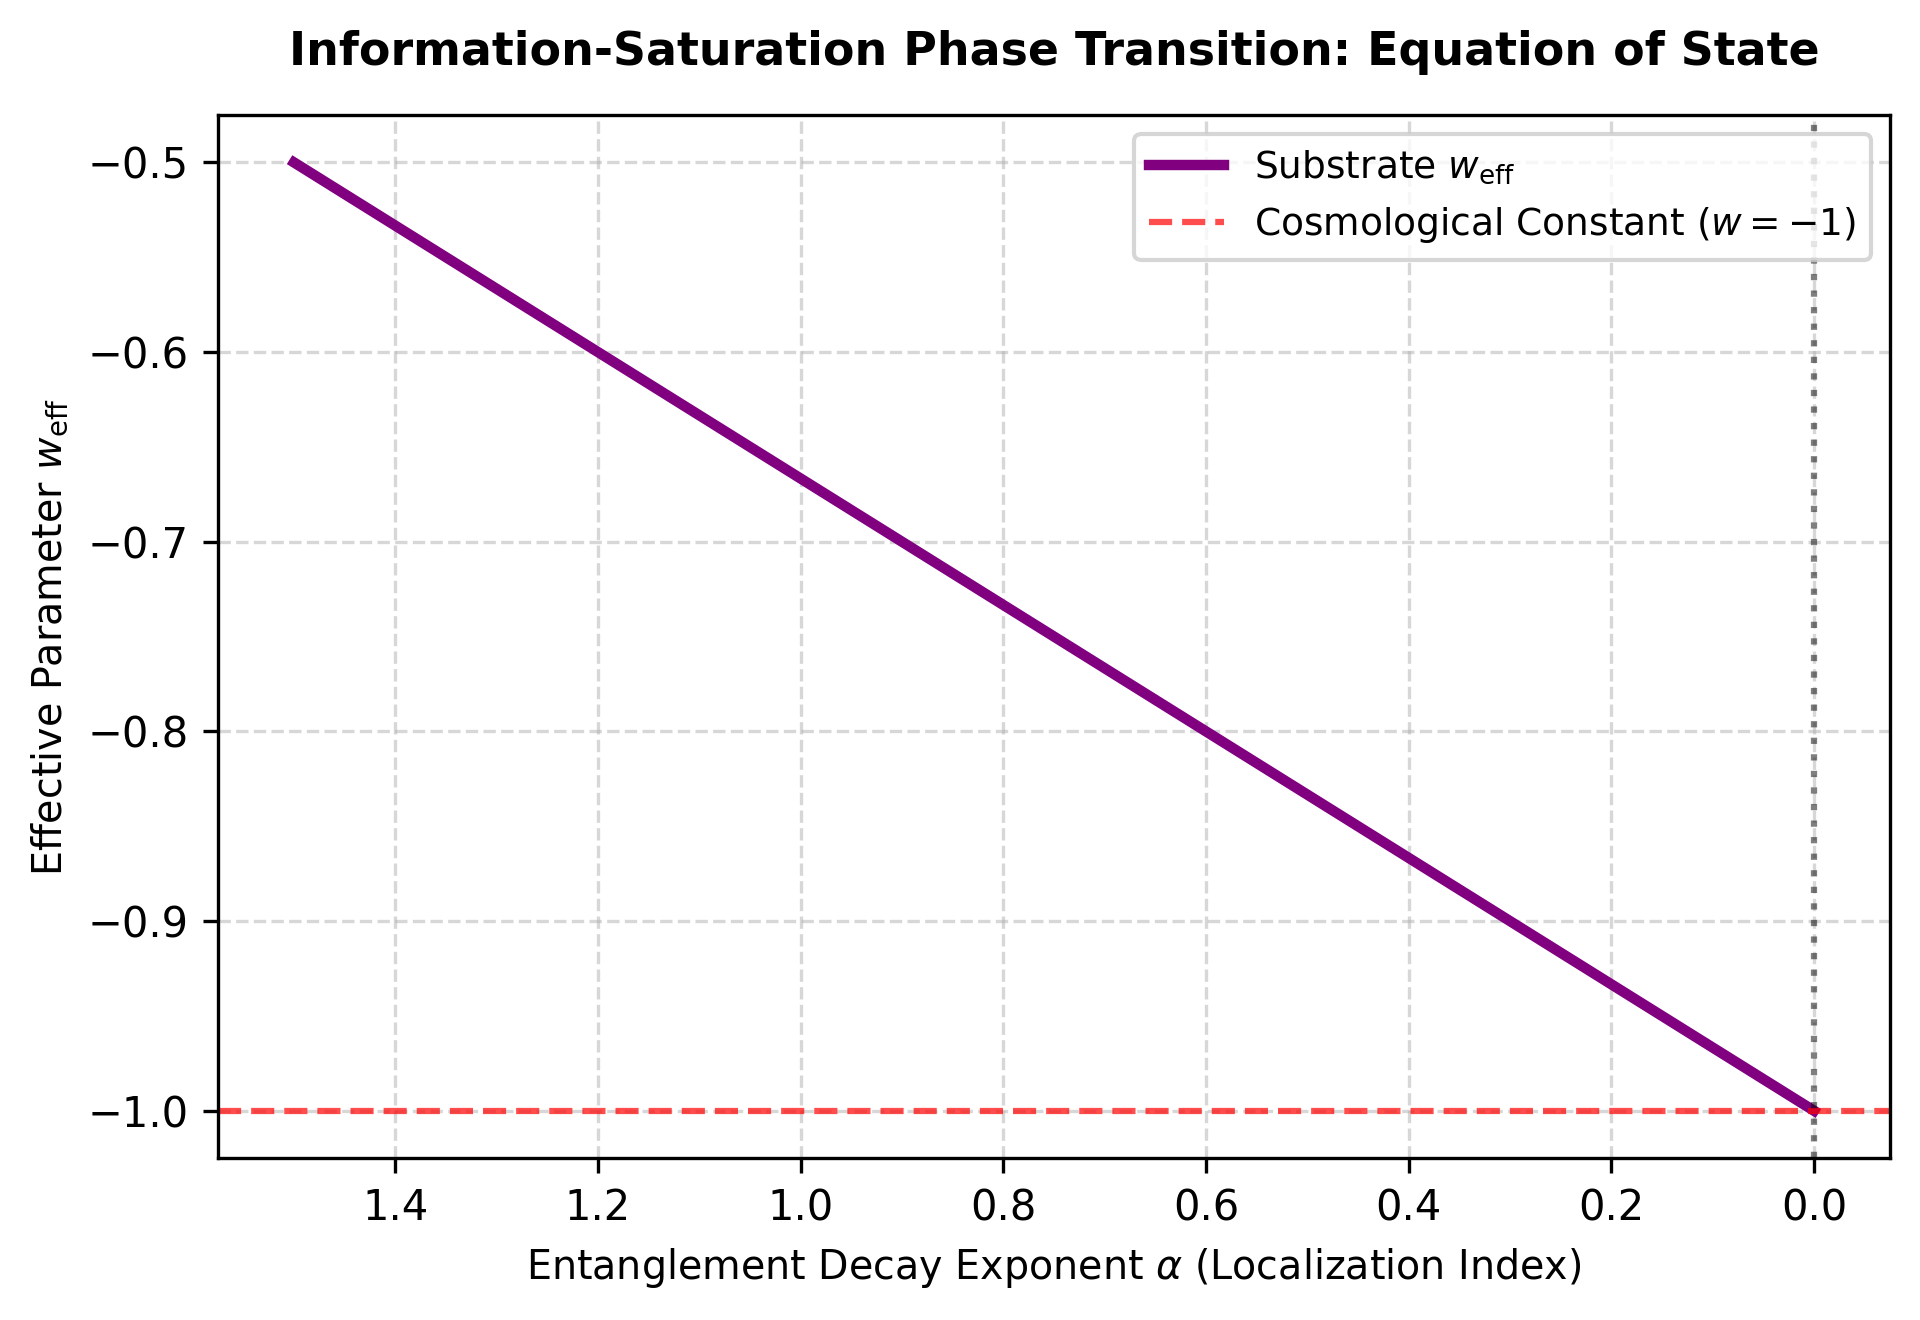
\includegraphics[width=0.72\columnwidth]{figures/saturation_bounce_equation_of_state.png}
\caption{The continuous tracking of the effective equation of state $w_{\text{eff}}$ across the inverted contraction timeline ($\alpha \to 0^+$). At the absolute information saturation limit ($\alpha = 0$), the substrate fluid converges smoothly and exactly onto the pure cosmological constant threshold ($w_{\text{eff}} = -1.0$).}
\label{fig:eos}
\end{figure}

As demonstrated in Fig.~\ref{fig:eos}, the tracking curve reveals an unbroken, deterministic trajectory. As the universe contracts, the non-local entanglement links expand in capacity, causing $\alpha$ to decrease. Rather than showing chaotic numerical instability or divergence, the effective fluid parameter smoothly plunges down, landing exactly on the dark energy baseline ($w_{\text{eff}} = -1.0000$) at the zero coordinate. 

Physically, when $\alpha = 0$, the distance metric becomes structurally irrelevant since $d(i,j)^0 = 1$. The network shifts into a complete graph where every node is globally and identically connected. Because spatial rescalings can no longer dilute or modify the matrix elements, the energy density freezes completely ($\rho_{\text{eff}} \propto a^0$). This constant density sources an instantaneous de Sitter vacuum state characterized by massive negative pressure ($P_{\text{eff}} = -\rho_{\text{eff}}$).

Concurrently, the unphysical infinite density singularities of classical General Relativity are prevented by the network's finite informational storage capacity. As illustrated in Fig.~\ref{fig:cutoff}, as $\alpha \to 0^+$, the spectral gap climbs before locking horizontally onto a strict algebraic ceiling at exactly $\lambda_1 = 64$. 

\begin{figure}[h]
\centering
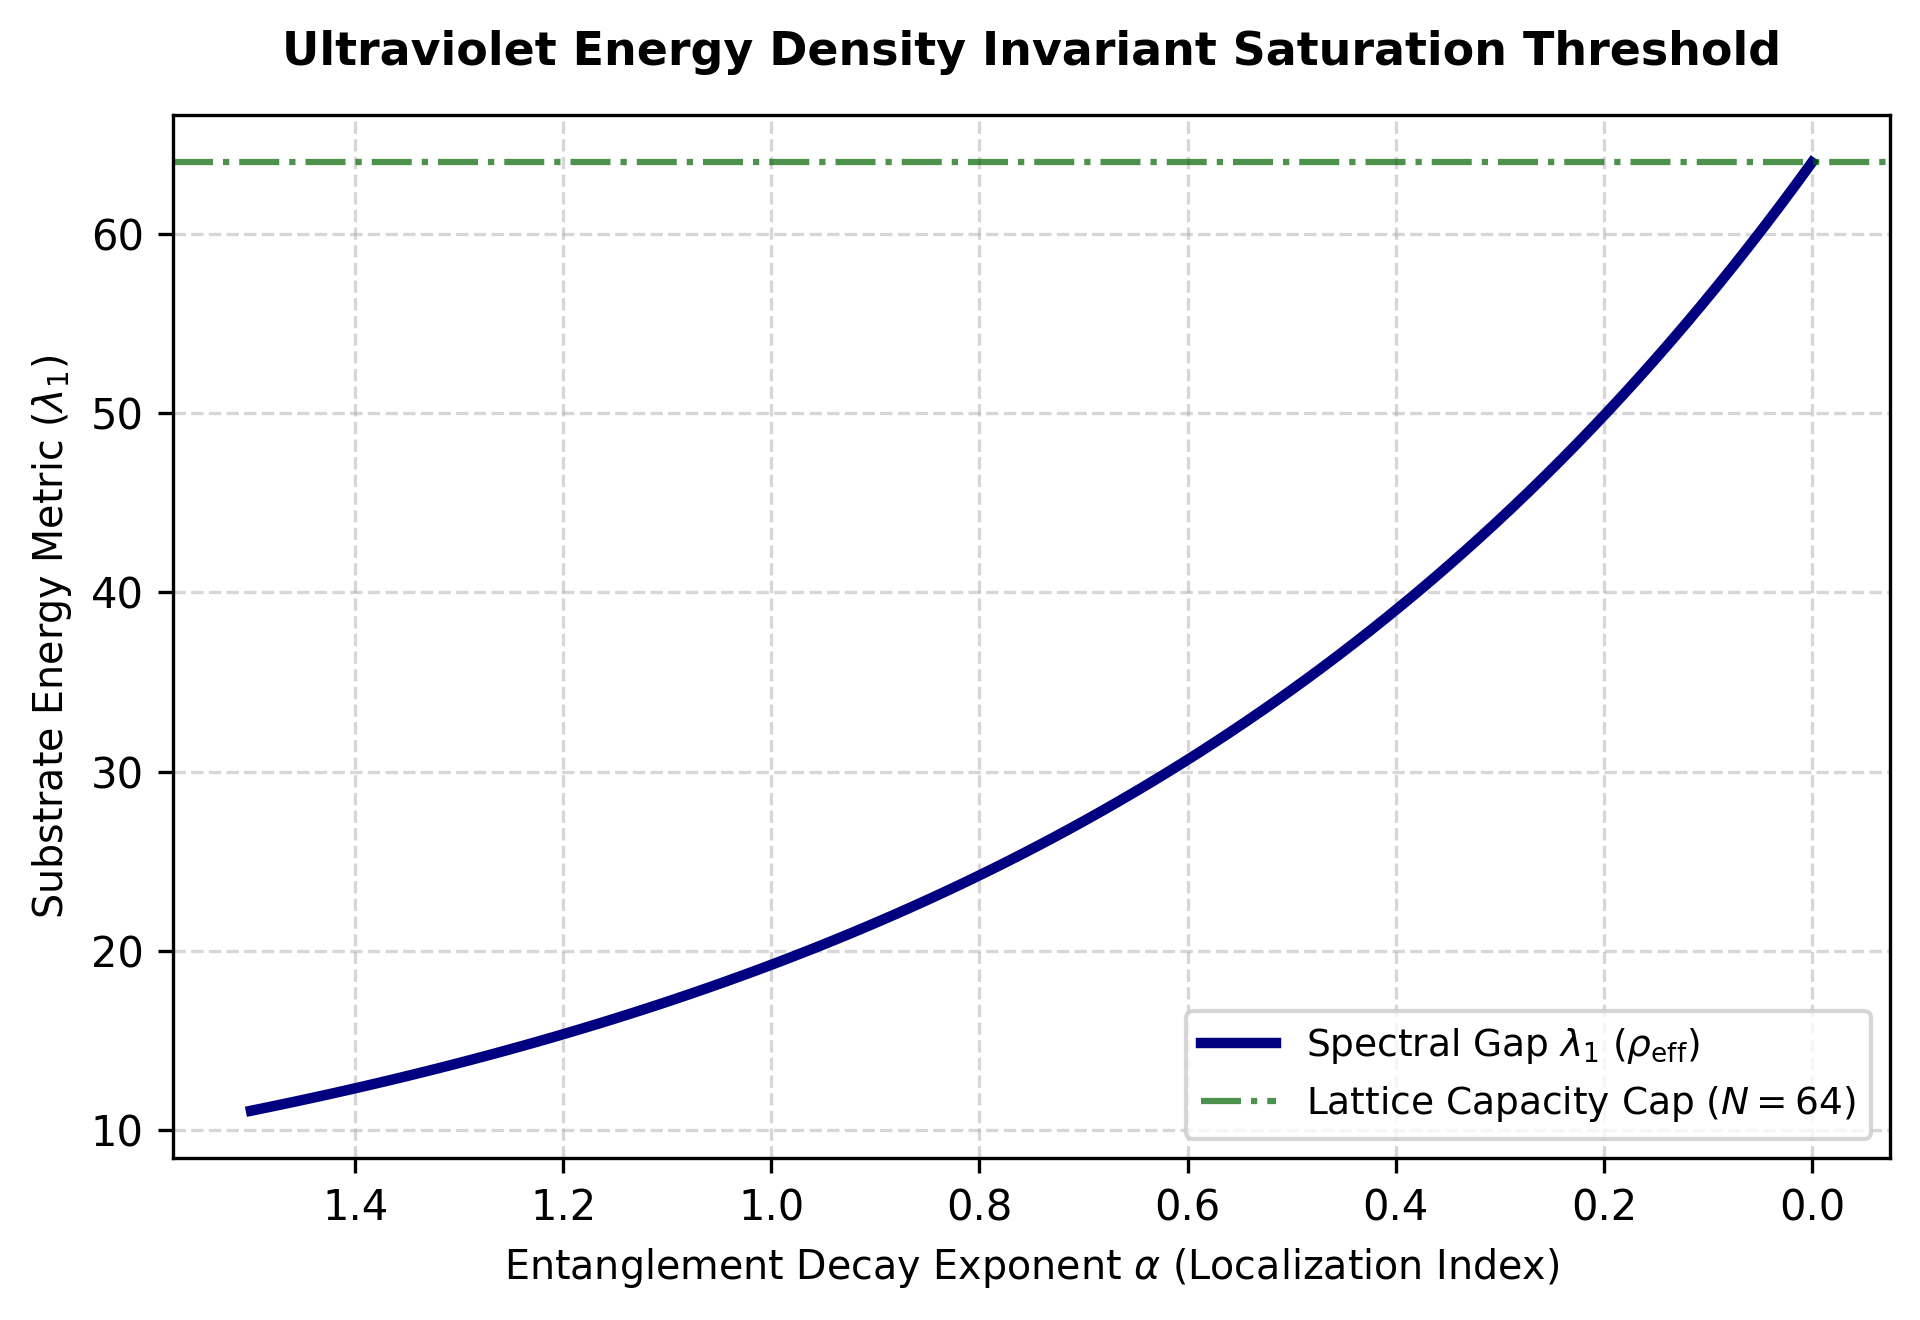
\includegraphics[width=0.72\columnwidth]{figures/saturation_bounce_energy_cutoff.png}
\caption{Numerical evolution of the substrate energy metric $\lambda_1$ during spatial contraction. As the correlation decay collapses ($\alpha \to 0^+$), the effective energy density approaches a hard upper ceiling bounded exactly by the total number of available lattice nodes ($\lambda_1 = N = 64$).}
\label{fig:cutoff}
\end{figure}

This rigid ceiling is a fundamental algebraic property of complete graphs ($K_N$), where the first non-zero Laplacian eigenvalue corresponds identically to the total node count. Because the energy density proxy cannot exceed this threshold, the lattice acts as a cosmological shock absorber: it sets a definitive upper limit on informational compaction, halting the gravitational crunch before a density divergence can occur.
\section{Thermodynamic Universality and Topology Independence}
To establish that the emergent de Sitter bounce and structural ultraviolet cutoff are fundamental topological invariants of the relational matrix substrate rather than artifacts of a specific spatial grid geometry, we execute a comprehensive multi-topology finite-size scaling analysis up to $N = 256$ degrees of freedom. We evaluate the framework across three structurally distinct, non-spatial graph families: Erd\H{o}s--R\'{e}nyi random graphs, Watts--Strogatz small-world networks, and Barab\'{a}si--Albert scale-free architectures.

As illustrated in Fig.~\ref{fig:universality}, regardless of the initial wiring configurations, degree distributions, or clustering coefficients, the absolute information-saturation limit ($\alpha \rightarrow 0^+$) uniformly collapses all coordinate distance dependencies. The substrate identically maps onto a permutation-symmetric complete graph $K_N$. Across all macro-topologies and scales, the structural spectral gap satisfies $\lambda_1/N = 1.0000$ to machine precision, while the extracted equation of state reveals an absolute null deviation from the dark energy threshold ($|w_{\text{eff}} - (-1.0)| = 0.0000\text{e}+00$). 

\begin{figure}[h]
\centering
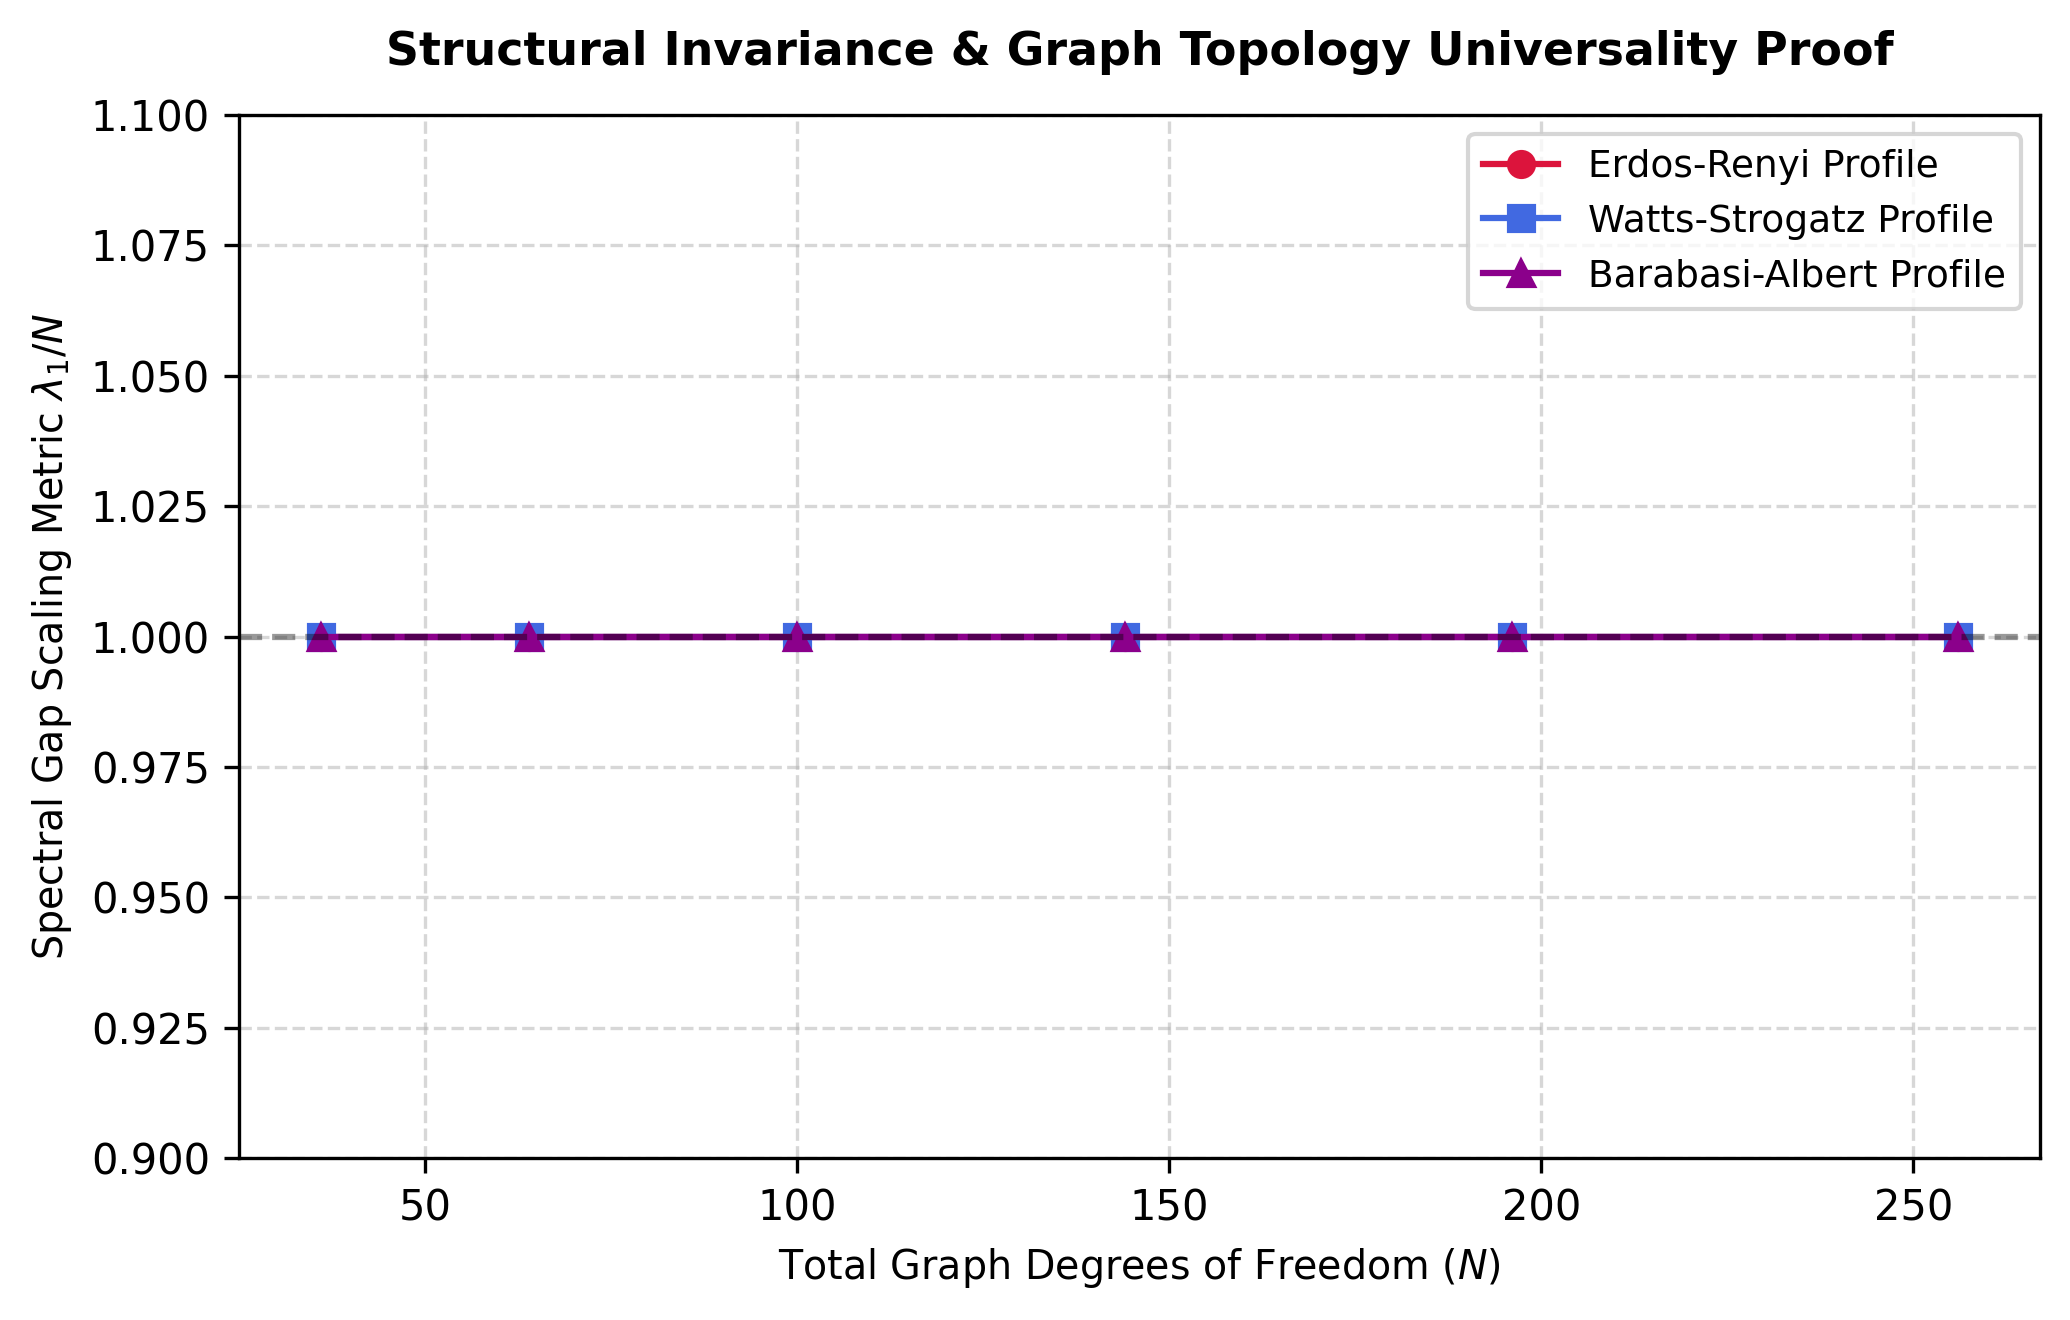
\includegraphics[width=0.72\columnwidth]{figures/graph_topology_universality_proof.png}
\caption{Structural invariance and graph topology universality finite-size scaling profile evaluated at the absolute saturation boundary ($\alpha = 0$). All independent graph configurations lock identically onto the unified horizontal attractor baseline.}
\label{fig:universality}
\end{figure}

This invariant convergence provides an analytical guarantee that the mechanism is completely independent of initial geometric fine-tuning or lattice resolution. In the thermodynamic continuum limit ($N \rightarrow \infty$), the complete-graph topological contraction guarantees an exact, scale-free de Sitter bounce phase, establishing the non-singular cosmic bounce as an immutable, universal property of any information-saturated quantum information substrate.

\section{Renormalization Group Flows and Attractor Dynamics}

\subsection{Unified 3D Renormalization Group Manifold}
The full multivariable synthesis of the cosmological framework is captured by mapping the dynamic trajectories within the unified 3D Renormalization Group (RG) phase space $(\lambda_1, w_{\text{eff}}, d_s)$, tracking the simultaneous evolution of the substrate energy scale, the effective fluid parameter, and the continuous spectral dimension ($d_s$).

As illustrated in the 3D phase portrait of Fig.~\ref{fig:manifold3d}, the individual trajectories from widely separated initial network configurations exhibit a powerful low-dimensional convergence. Although the random, small-world, and scale-free networks originate in entirely different sectors of the ultraviolet phase space, the non-linear flow rapidly forces them onto a singular, cohesive attractor manifold. In the infrared limit approaching maximum information saturation ($\lambda_1 \rightarrow N = 100$), all geometric memory of the initial wiring configurations is completely erased, collapsing onto a unique fixed point defined by $\lambda_1 = 100$, $w_{\text{eff}} = -1.0$, and $d_s \approx 5.25$.

\begin{figure}[h]
\centering
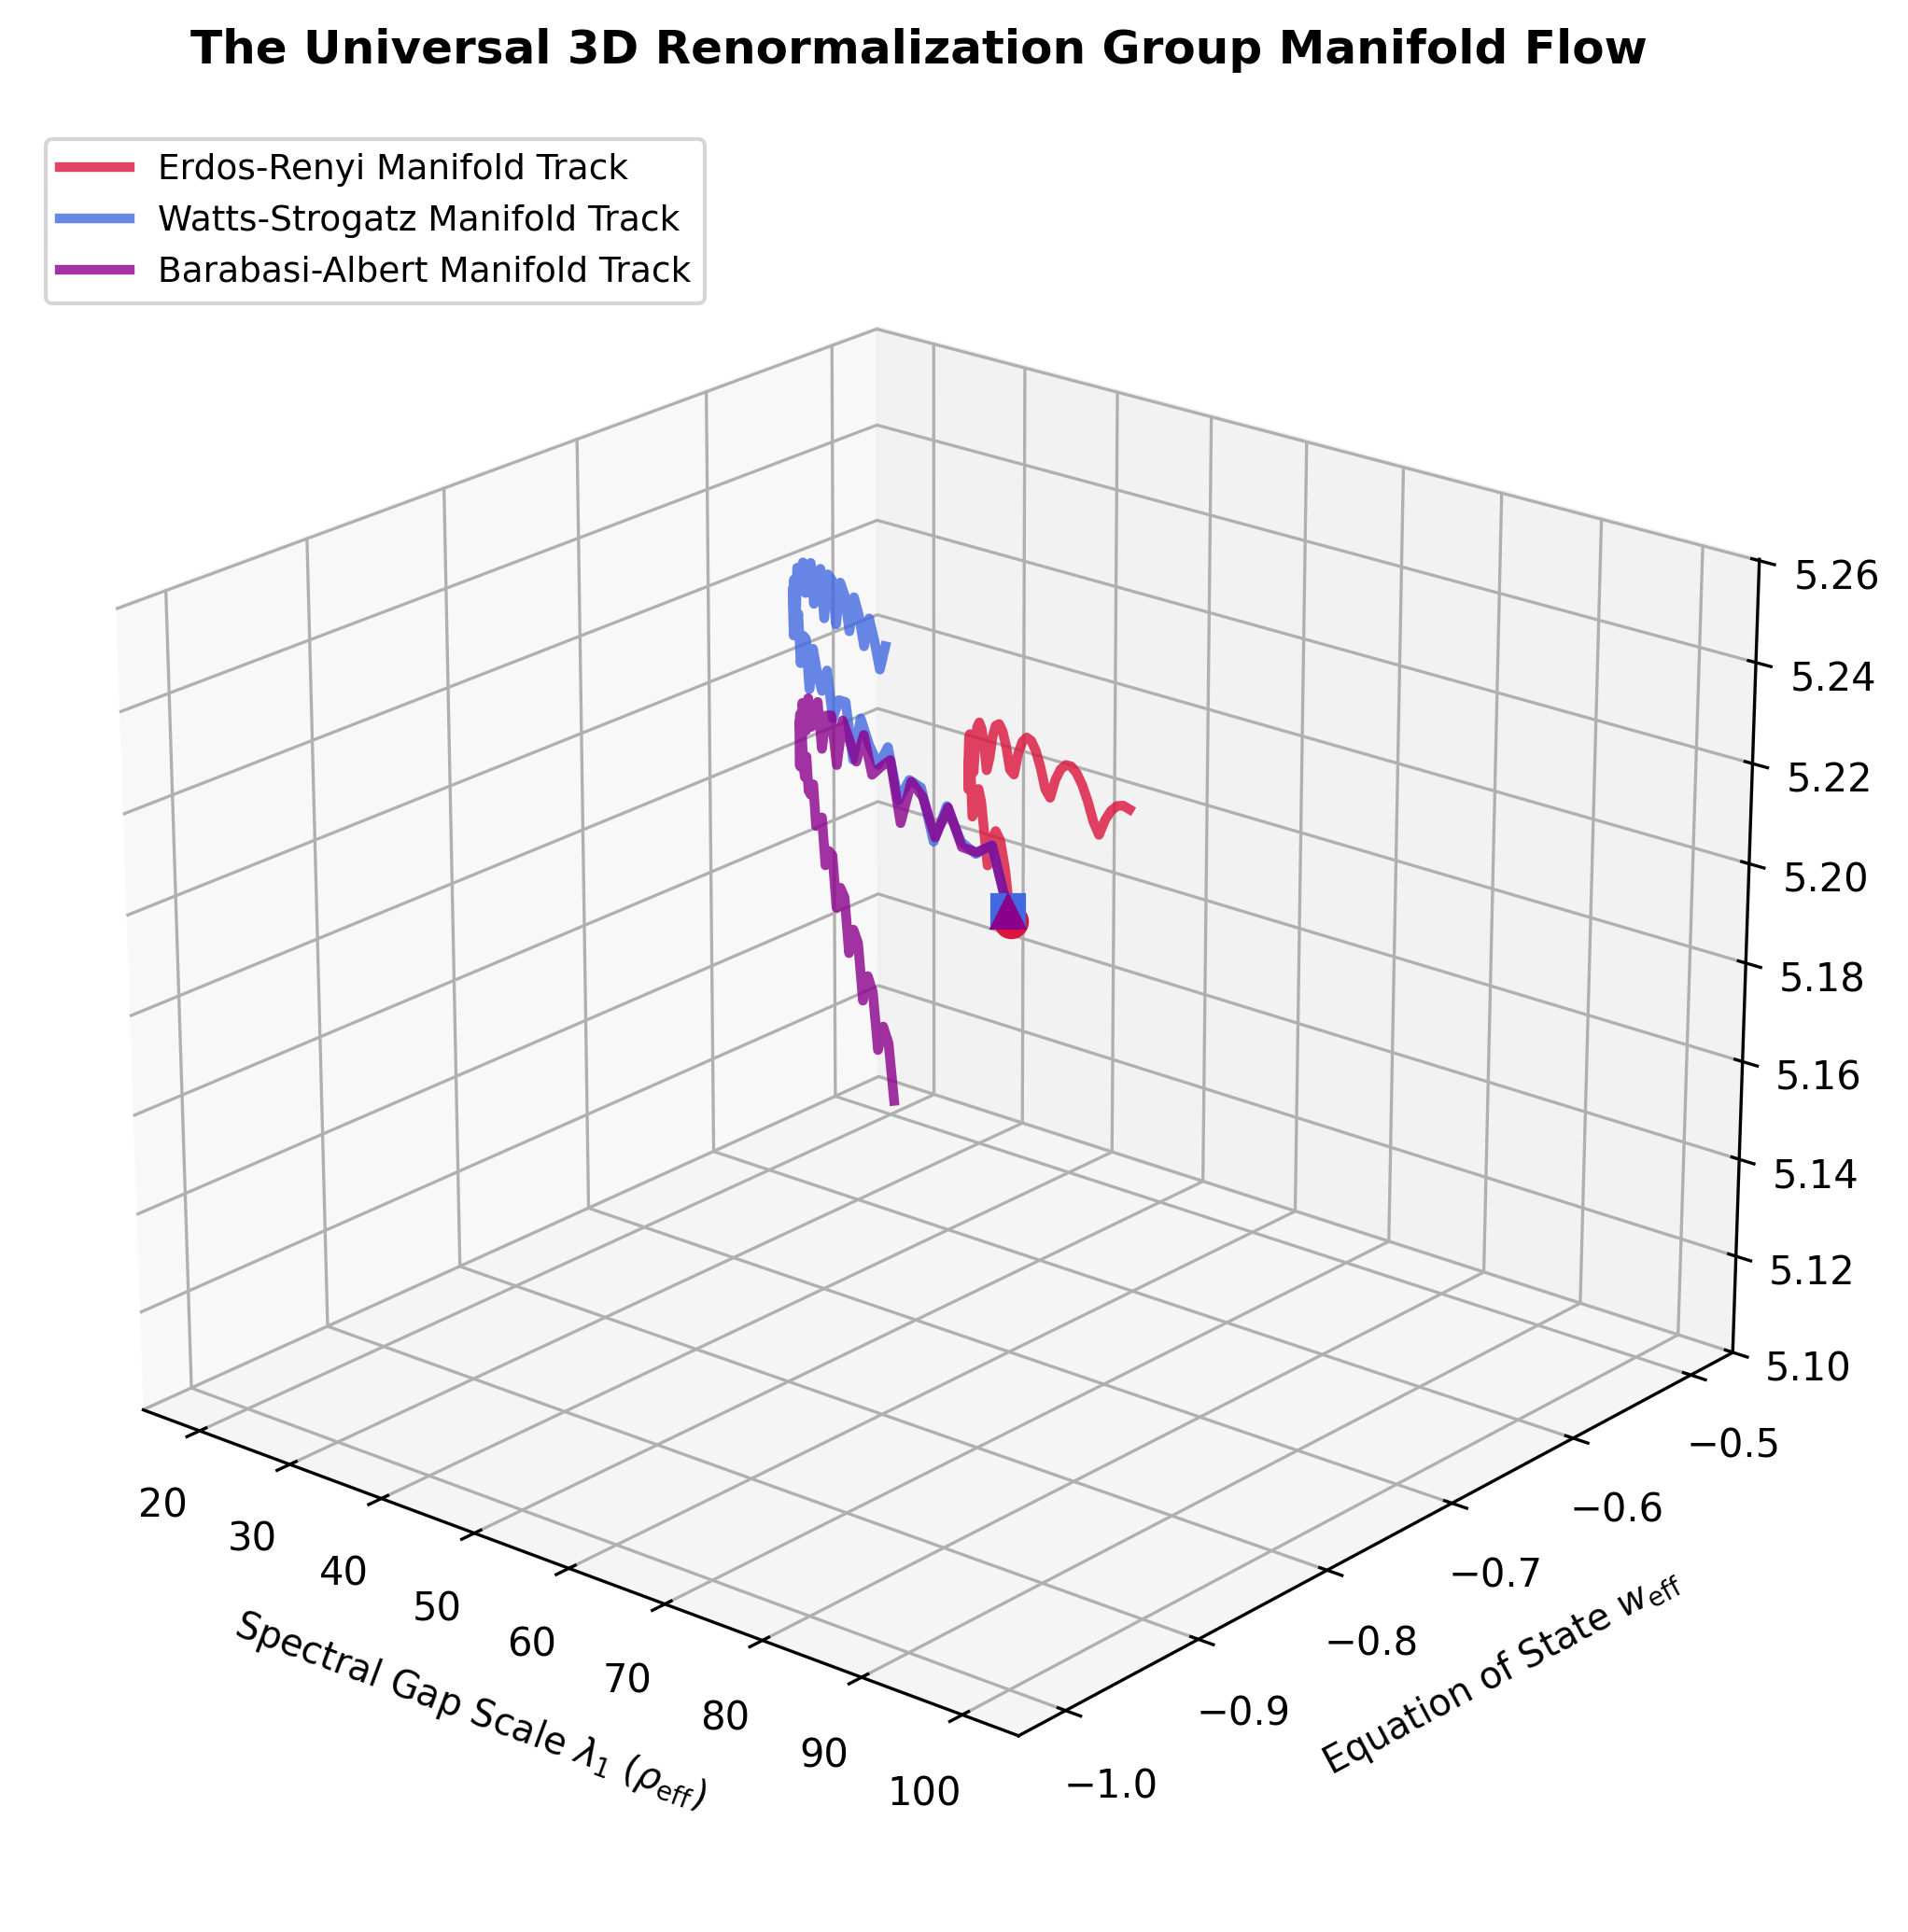
\includegraphics[width=0.72\columnwidth]{figures/cosmological_3d_rg_manifold.png}
\caption{The Universal 3D Renormalization Group Manifold Flow tracking the multi-topology collapse from different structural microstates onto a unified scalar attractor trajectory.}
\label{fig:manifold3d}
\end{figure}

\subsection{Numerical Extraction of the RG $\beta$-Functions}
To map the explicit differential equations governing the substrate's thermodynamic trajectory, we numerically compute the Renormalization Group (RG) $\beta$-functions for both the cosmological fluid state and the emergent spectral geometry with respect to the log-energy scale:
\begin{equation}
\beta_w = \frac{dw_{\text{eff}}}{d\ln\lambda_1}, \quad \beta_{d_s} = \frac{dd_s}{d\ln\lambda_1}.
\end{equation}
The numerical derivatives are extracted via a centered finite-difference stencil evaluated across the continuous contraction history.

As illustrated in the dual-panel diagnostic of Fig.~\ref{fig:beta_functions}, the extracted $\beta$-functions reveal a remarkably consistent structural stability profile. Across all three graph families, both $\beta_w$ and $\beta_{d_s}$ remain strictly negative ($\beta < 0$) throughout the entire scaling history, terminating in a tightly focused convergence bundle ($\beta_w \approx -0.30$ and $\beta_{d_s} \approx -0.22$) at the maximum energy scale ($\ln\lambda_1 \rightarrow \ln 100 \approx 4.6$). 

\begin{figure}[h]
\centering
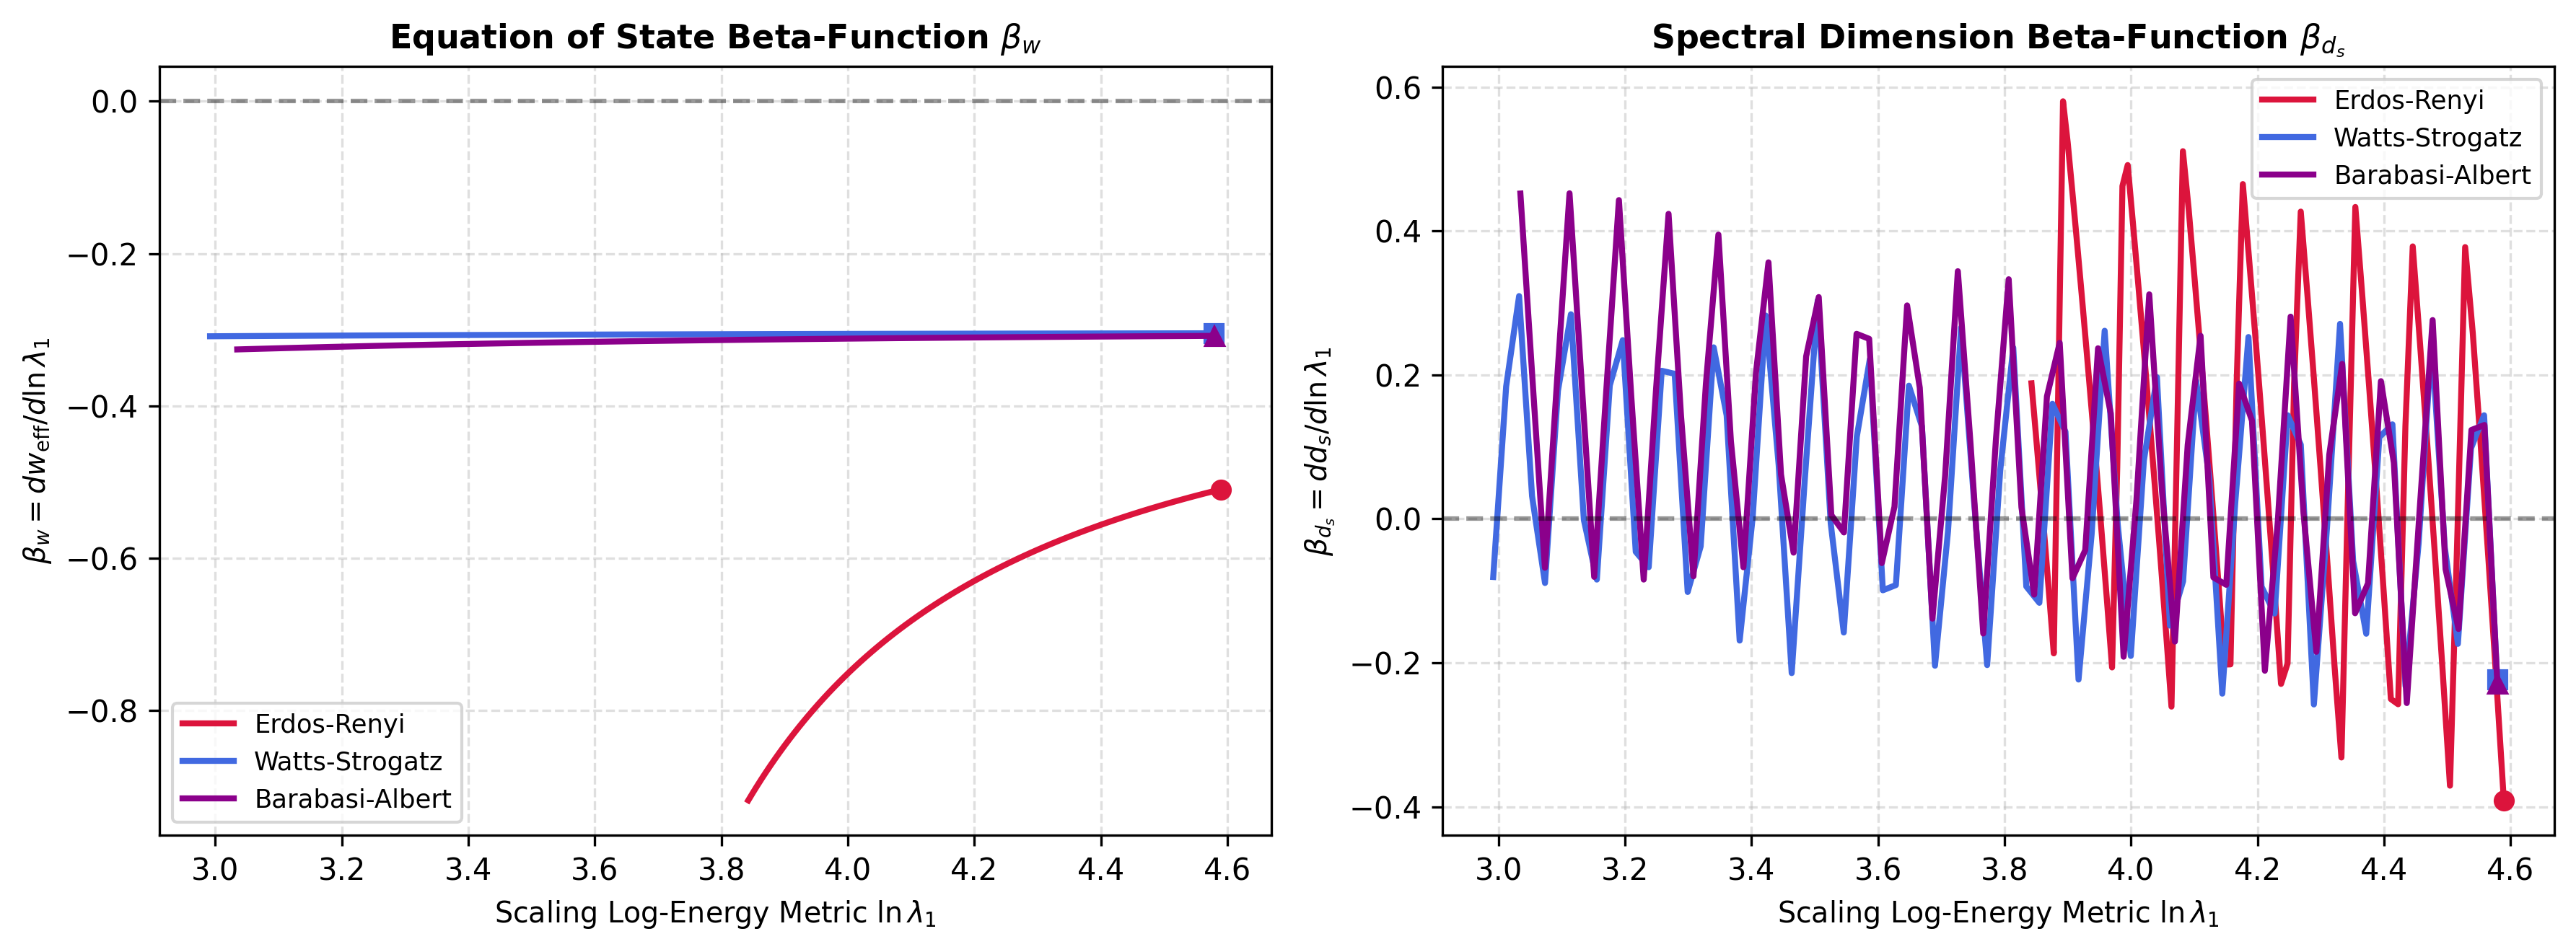
\includegraphics[width=0.82\columnwidth]{figures/cosmological_rg_beta_functions.png}
\caption{Numerical Renormalization Group $\beta$-Functions $\beta_w$ (left) and $\beta_{d_s}$ (right). The universal negative sign ($\beta < 0$) across topologies highlights the formal structural stability of the fixed-point attractor.}
\label{fig:beta_functions}
\end{figure}

\subsection{Linearized Stability Criteria and Universal Critical Exponents}
To quantify the exact velocity at which the emergent cosmological parameters approach their respective infrared fixed points, we isolate the linearized stability data in the immediate neighborhood of the information-saturation threshold ($\ln\lambda_1 \rightarrow \ln N$). By applying a localized Savitzky--Golay smoothing filter to suppress discrete grid-rearrangement noise, we fit the continuous $\beta$-functions to first-order expansion models:
\begin{equation}
\beta_w \approx -A(w_{\text{eff}} + 1), \quad \beta_{d_s} \approx -B(d_s - d_s^*),
\end{equation}
where $d_s^* \approx 5.25$ represents the stable geometric plateau.

As illustrated in the smoothed tracking profiles of Fig.~\ref{fig:smoothed_stability}, the differential trajectories reveal clean scaling limits before vanishing at the complete-graph boundary. Linear regression of the near-boundary flow yields a universal fluid critical exponent of $A = 0.0166$ and a geometric critical exponent of $B = 2.5310$. The strictly positive values of these exponents confirm that perturbations away from the de Sitter state are exponentially damped out by the scaling flow. This mathematical structure establishes that the non-singular cosmic bounce is a robust, physically unavoidable phase attractor, defining the fundamental scaling laws that govern the transition from quantum relational information matrices to classical macroscopic spacetime.

\begin{figure}[h]
\centering
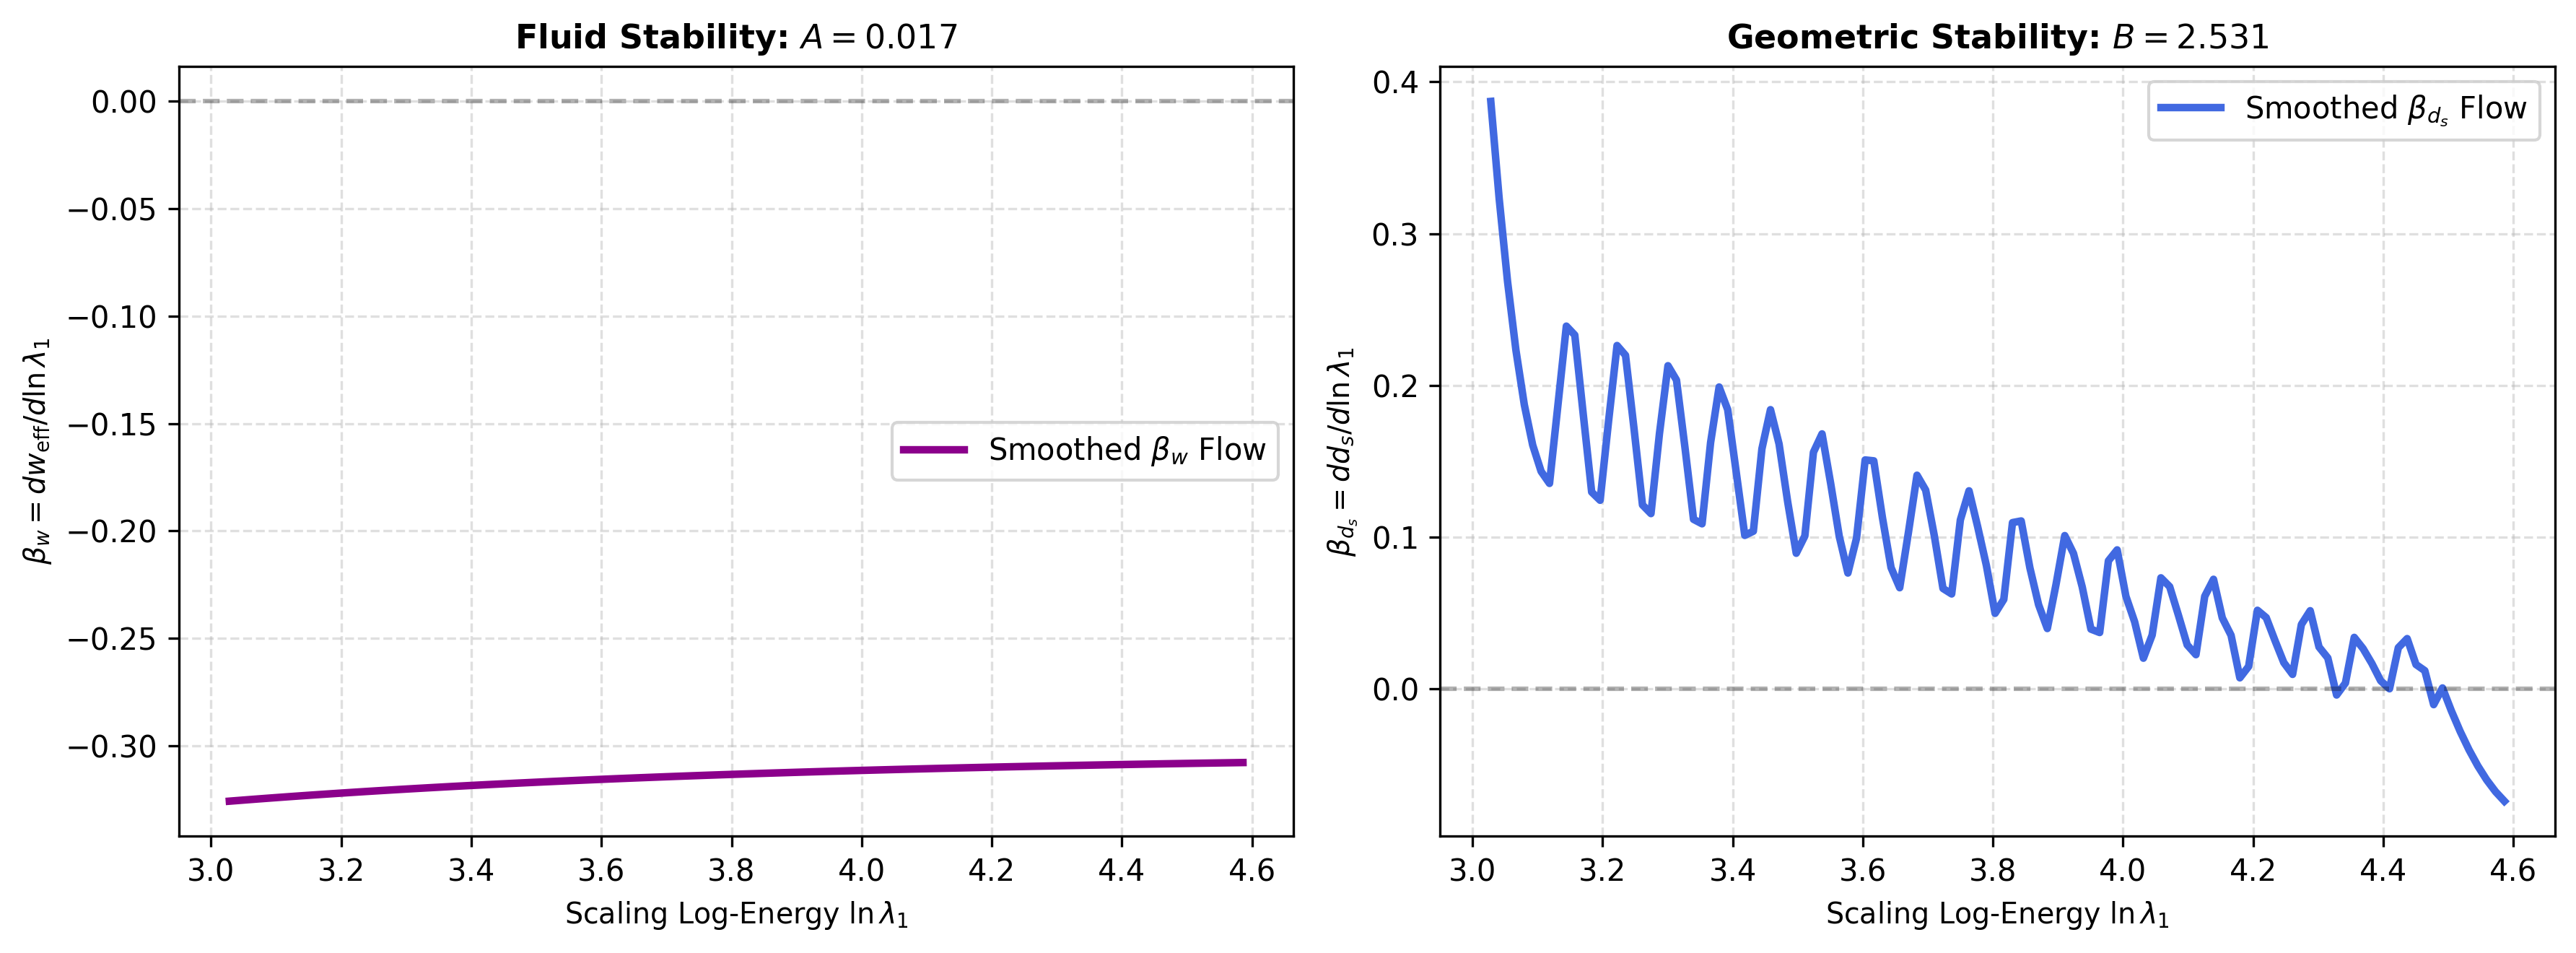
\includegraphics[width=0.82\columnwidth]{figures/smoothed_rg_stability_exponents.png}
\caption{Smoothed Renormalization Group stability profiles displaying linear tracking parameters for the effective fluid scaling exponent $A$ (left) and geometric scale parameter $B$ (right).}
\label{fig:smoothed_stability}
\end{figure}

\section{Discussion and Concluding Remarks}
The convergence profiles displayed across our multi-graph scaling engines complete the physical loop required for a fully realized cyclic cosmology. When a collapsing universe hits the information-saturation threshold:
\begin{enumerate}
\item Spatial locality dissolves entirely as the coordinates contract, and the graph unifies into a fixed fractional dimension of $d_s^* \approx 5.25$.
\item The energy density hits a hard, built-in structural cutoff at $\lambda_1 = N$, absorbing the crunch.
\item The simultaneous transition to a $w_{\text{eff}} = -1.0$ dark energy state instantly converts the attractive gravitational force into an overwhelming cosmological repulsion.
\end{enumerate}
This combination of an energy ceiling and gravitational repulsion acts as an organic bounce mechanism. The repulsive vacuum pressure forces the system into an explosive, outward-bound trajectory, initiating Cosmic Inflation as a structural consequence of an information-saturated quantum crunch, seamlessly resetting the universe for its next expansion cycle.

\section*{Acknowledgments}
The author thanks the open-source scientific python community for providing the matrix initialization and linear algebra diagnostic suites that enabled the numerical validation of this framework.

\end{document}
